\documentclass[a4paper,addpoints,12pt]{exam}
 
\usepackage[utf8]{inputenc} 
\usepackage[left=12mm,right=15mm,top=20mm,bottom=30mm]{geometry}
\usepackage{xcolor}
\usepackage[most]{tcolorbox}
\usepackage{changepage}

%details
\newcommand{\modulecode}{Mathématiques}
\newcommand{\papertitle}{Devoir Surveillé}
\newcommand{\detfilla}{Nom :}
\newcommand{\detfillb}{Numéro  :}
\newcommand{\detfillc}{Classe :}
\newcommand{\examtime}{1 heure}
\newcommand{\examdate}{1\textsuperscript{st} October 2020}
\newcommand{\classename}{1.A.C}
\newcommand{\extrapages}{3}


%Reformats questions and parts
\renewcommand{\questionlabel}{\textbf{\thequestion.}}
\renewcommand{\partlabel}{\textbf{(\thepartno)}}
\renewcommand{\subpartlabel}{\textbf{\thesubpart)}}


%Defines dotted line for answer
\def\dotfill#1{\cleaders\hbox to #1{.}\hfill}
\newcommand\dotline[2][.5em]{\leavevmode\hbox to #2{\color{gray}\dotfill{#1}\hfil}}


%MACROs for answer line
\newcommand{\ans}[1]{\vspace*{#1}
\begin{flushright}\dotline[2pt]{35mm}\end{flushright}
\droppoints}

\newcommand{\ansline}[1]{\vspace*{#1}
\begin{flushright}\dotline[2pt]{35mm}\end{flushright}
\droppoints
\fullwidth{\noindent\color{gray}\rule{\textwidth}{1pt}}}

%Header and footer
\definecolor{washoutgrey}{RGB}{140,140,140}
\definecolor{lightgrey}{RGB}{240,240,240}

\pagestyle{headandfoot}

\runningheadrule

\runningfootrule

\runningheader{\textcolor{washoutgrey}{\textbf{\modulecode}}}{\includegraphics[width=.2\textwidth]{Images/IMAGEHeader.png}}{\textcolor{washoutgrey}{\textbf{\papertitle}}}

\firstpagefooter{\includegraphics[width=.3\textwidth]{Images/IMAGEWebAddress.png}}{}{\vspace*{-10mm}\includegraphics[width=.1\textwidth]{Images/IMAGEFooterIcon.png}}

\runningfooter{\includegraphics[width=.3\textwidth]{Images/IMAGEWebAddress.png}}{\vspace*{-8mm}\textcolor{washoutgrey}{\textbf{Page \thepage\ of \pageref{lastpage}}}}{\begin{tcolorbox}[enhanced,colback=white,colframe=washoutgrey,hbox]{\hspace*{20mm}\textcolor{washoutgrey}{\large\textbf{/\pointsonpage{\thepage}}}}\end{tcolorbox}}


%extra answer pages

\newcommand{\notes}[3][\empty]{%
    \foreach \n in {1,...,#2}{%
        \ifthenelse{\equal{#1}\empty}
        {\dotline[2pt]{#3}\\}
        {\dotline[2pt]{#3}\vspace{#1}\\}
    }
}

\newcommand{\extraanswerpage}[1]{%
    \foreach \n in {1,...,#1}{%
        \newpage
        \begin{center}
            \begin{tcolorbox}[enhanced,colback=white,colframe=black]
            {\begin{center}\large \textbf{ADDITIONAL ANSWER PAGE:} Clearly number each question\end{center}}
            \end{tcolorbox}
        \end{center}
        \noindent
        \notes[10pt]{25}{\textwidth}
    }
}




%%%%%%%%%%%%%%%%%%%%%%%%%%%%%%%%%%%%%%%%%%%%%%%%%%%%%%%%%%%%%%

\begin{document}


%title page
\begin{tcolorbox}[colback=lightgrey,colframe=black,arc=1mm]

\begin{minipage}{.6\textwidth}
  \begin{tcbraster}[raster columns=1, raster column skip=0pt, raster equal height, colback=white, before skip=0pt]
    
    \begin{tcolorbox}[coltitle=black, enhanced jigsaw, boxrule=2pt ,segmentation style={solid,black,line width=2pt},sidebyside,lefthand width=1.5cm]
        \begin{large}\textbf{\detfilla}\end{large}
    \end{tcolorbox}
   
     \end{tcbraster}
\end{minipage}
\begin{minipage}{.4\textwidth}
     \begin{tcolorbox}[coltitle=black, enhanced jigsaw, boxrule=2pt ,segmentation style={solid,black,line width=2pt},sidebyside,lefthand width=3cm]
        \begin{large}\textbf{\detfillb}\end{large}
    \end{tcolorbox} 
    
\end{minipage}
 
    \vspace*{2mm}
    
    \begin{minipage}{.7\textwidth}
    
    \begin{tcbraster}[raster columns=1, raster column skip=0pt, raster equal height, colback=white, before skip=0pt]
    
    \begin{tcolorbox}[enhanced jigsaw, fontupper=\bfseries, colback=white, boxrule=2pt, segmentation style={solid,black,line width=2pt}]
        
        \begin{huge}
        \textbf{\modulecode}
        \end{huge}
        
        \vspace*{2mm}
        
        \begin{large}\textbf{\papertitle}\end{large}\hfill\textbf{\examdate}
        
        \tcblower
        
        \begin{large}
        \textbf{Durée: \examtime}\hfill\textbf{\classename}
        \end{large}
        
        
        
    \end{tcolorbox}
    
    \end{tcbraster}
    
    \end{minipage}%
    \begin{minipage}{.3\textwidth}
    
    \begin{adjustwidth}{10mm}{0mm}
    
    \begin{tcbraster}[raster columns=1, raster column skip=0pt, raster equal height, colback=white, before skip=0pt]
    
    \begin{tcolorbox}[enhanced jigsaw, fontupper=\bfseries, colback=white, boxrule=2pt, segmentation style={solid,black,line width=2pt}]
    
    \begin{huge}\textbf{Note}\end{huge}
    
    \tcblower
    
    {\hspace*{15mm}\begin{Huge}\textbf{/\numpoints}\end{Huge}}
        
    \end{tcolorbox}
    
    \end{tcbraster}
    
    \end{adjustwidth}
    
    \end{minipage}
    
    \vspace*{5mm}
    
\end{tcolorbox}


\vspace*{3mm}

%instructions
\begin{adjustwidth}{0mm}{-10mm}
\begin{minipage}{\textwidth}

\begin{small}

\textbf{Instructions to candidates}

\begin{itemize}
\item This question book consists of \textbf{\numquestions\ questions}. You must attempt \textbf{ALL} questions.
\item The maximum mark for the whole paper is \textbf{\numpoints} 
\item The use of a scientific calculator \textbf{IS} permitted.
\item At the start of the examination, you should have:
\begin{adjustwidth}{20mm}{}
\begin{itemize}    
\item[\textbullet] this question book    
\item[\textbullet] rough paper
\end{itemize}
\end{adjustwidth}
\item Read the task information carefully before you begin to write.
\item Write your answers in this question book.
\item If additional space is needed to complete your answer, additional paper is available at the end of this question book. Clearly write the number of the question that you are answering on this additional paper.
\item Diagrams should be drawn in pencil. All other working should be written in blue or black ink. Do not write working in pencil.\item Any working that you do not wish to be marked should be crossed out with a single line.
\item If you have any questions at any time during the examination, you must raise your hand and wait for an invigilator. \textbf{DO NOT} attempt to communicate, by any means, with any other candidate at any time before or during the examination.
\item At the end of the examination, \textbf{DO NOT} speak or leave your seat until you have handed this question book to an invigilator and you have been told by an invigilator that you may leave the room.
\end{itemize}

\end{small}
\end{minipage}%
\begin{minipage}{.1\textwidth}
\vspace*{-50mm}\hspace*{-40mm}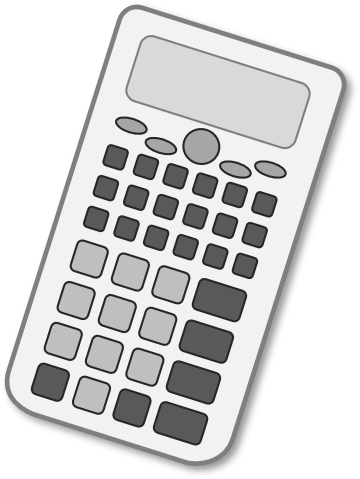
\includegraphics[width=1.5\textwidth]{Images/Calculator.png}
\end{minipage}
\end{adjustwidth}

\newpage

%questions

\begin{tcolorbox}[%
    enhanced,
    breakable,
    frame hidden,
    overlay broken={
        \draw[line width=0.5mm, gray, rounded corners]
        (frame.north west) rectangle (frame.south east);},colback=white,height fixed for=all]{}

\begin{questions}

\pointsdroppedatright
\marksnotpoints
\marginpointname{ \points}
\setlength{\rightpointsmargin}{25mm}
\pointformat{\bfseries\boldmath[\themarginpoints]}

\question[4] Find the equation of the tangent to $y=4x^2-5x+7$\ans{100mm}

\question Solve
\begin{parts}
\part[2] $3(x-2)=1$\ans{20mm}
\part[4] $\displaystyle 5x-4=\frac{1}{2}$\ansline{30mm}
\end{parts}

\newpage

\question Simplify
\begin{subparts}
\subpart[1] $5(x+4)$\droppoints
\subpart[4] $\displaystyle \frac{1}{x+4}-\frac{3x}{x-2}$\\

\fullwidth{\notes[10pt]{3}{\textwidth}}

\droppoints
\end{subparts}

\newpage

\question[5] \hfill
\begin{center}
    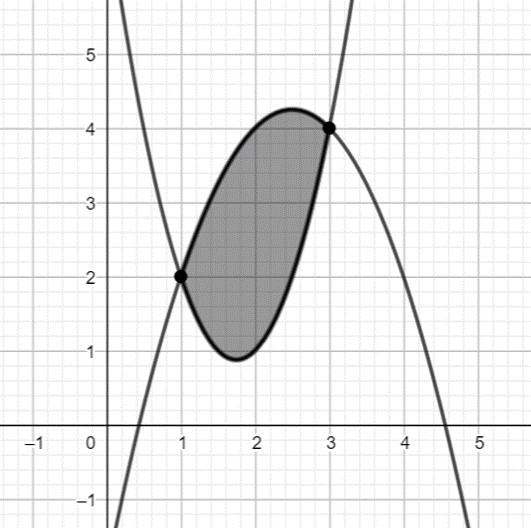
\includegraphics[width=.5\textwidth]{Images/ExampleGraph.png}
\end{center}

The graph below shows the curves $y=-x^2+5x-2$ and $y=2x^2-7x+7$\newline
Find the area of the shaded region.




\begin{center}
    \begin{tcolorbox}[enhanced,colback=white,colframe=black]
        {\begin{center}\Large \textbf{END OF EXAMINATION QUESTIONS}\end{center}}
    \end{tcolorbox}
\end{center}



\end{questions}

\extraanswerpage{\extrapages}

\label{lastpage}

\end{tcolorbox}

\end{document}